% ! TEX root = ../m1-19-20.tex

\chapter{Metoda celor mai mici pătrate}

Această metodă este strîns legată de conceptul de \emph{interpolare}, care
ne ajută să găsim cea mai potrivită curbă, pornind de la un set de puncte
(reprezentînd, eventual, date experimentale).

Cazul particular pe care îl vom discuta este acela al curbelor liniare,
deci atunci cînd se caută cea mai potrivită \emph{dreaptă} pentru un set
de puncte. Această dreaptă se mai numește \emph{dreaptă de regresie}
și spunem că ea \emph{mediază} între un set de puncte date, în sensul
că optimizează erorile.
\index{dreaptă!de regresie}

Pe scurt, dacă se dă un set de date experimentale, distribuite într-un
anume fel în plan și avem de găsit cea mai potrivită dreaptă care să
medieze între aceste puncte, sîntem în situația din figura \ref{fig:mcmmp}.

\begin{figure}[!htbp]
  \centering
  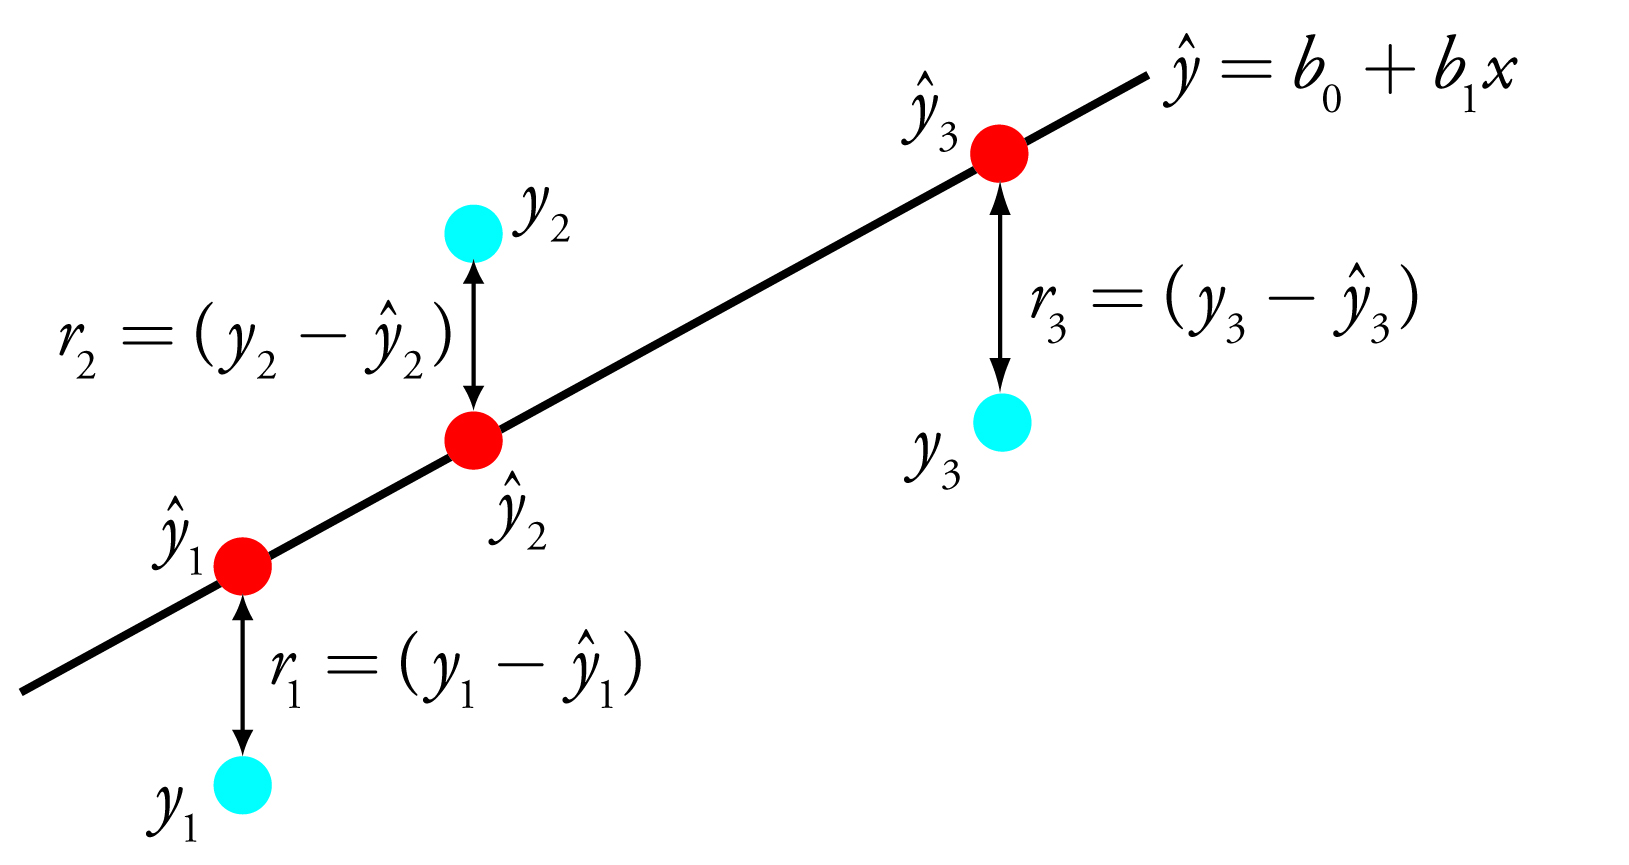
\includegraphics[scale=0.6]{fig/leastsquare.jpg}
  \caption{\emph{Dreapta $ \hat{y} = b_0 + b_1 x $ care mediază \\ %
      între punctele $ y_i $, cu calculul erorilor $ r_i $}}
  \label{fig:mcmmp}
\end{figure}

Această dreaptă se va găsi astfel încît \emph{suma pătratelor erorilor}
să fie minimă. Motivul simplu este că erorile pot fi și pozitive, și
negative, iar mai mult, erorile mari vrem să fie \qq{amplificate} de
metodă, erorile mai mici fiind de o importanță inferioară. De aceea,
metoda se numește \emph{metoda celor mai mici pătrate}.

Fie, deci, dreapta $ y = ax + b $, dreapta de regresie liniară pe care
o căutăm, care să medieze între punctele $ P_i(x_i, y_i) $.

Echivalent, putem scrie relația și funcțional, în sensul că dreapta
căutată se asociază unei funcții $ f(x) = ax + b $. Atunci,
dacă punctul $ P_i $ se găsește pe această dreaptă, are loc relația
$ f(x_i) = y_i $. Rezultă că eroarea poate fi calculată prin diferența
$ |y_i - f(x_i)| $ și vom fi interesați de suma pătratelor acestor erori.
Aceasta va fi funcția pe care încercăm să o minimizăm, iar argumentele sale
sînt coeficienții $ a, b $ care definesc dreapta căutată

Așadar, definim:
\[
  F(a, b) = \sum_i (f(x_i) - y_i)^2 = \sum_i (ax_i + b - y_i)^2.
\]

Metoda dorește, deci, să minimizeze eroarea, deci problema revine la a găsi
$ M(a, b) $ \emph{punctul de minim} al funcției $ F(a, b) $ de mai sus.
Coordonatele punctului vor defini dreapta de regresie căutată.

%%%%%%%%%%%%%%%%%%%%%%%%%%%%%%%%%%%%%%%%%%%%%%%%%%%%%%%%%%%%%%%%%%%%%%

\section{Exerciții}

Găsiți dreptele de regresie care mediază între punctele:
\begin{enumerate}[(a)]
\item $ (1, 3), (2, 4), (-1, 0) $;
\item $ (2, 3), (-1, -1), (0, 2) $;
\item $ (1, 0), (2, 1), (3, 2), (-1, 2) $;
\item $ (1, 1), (2, 1), (-1, 0), (-2, 1) $;
\item $ (1, 0), (2, 1), (-1, 1), (-2, -2) $.
\end{enumerate}



%%% Local Variables:
%%% mode: latex
%%% TeX-master: "../m1-19-20"
%%% End:
